\section{Physics Objects Reconstruction}
\subsection{Track and vertex}
\begin{figure}[bht]
    \begin{centering}	
    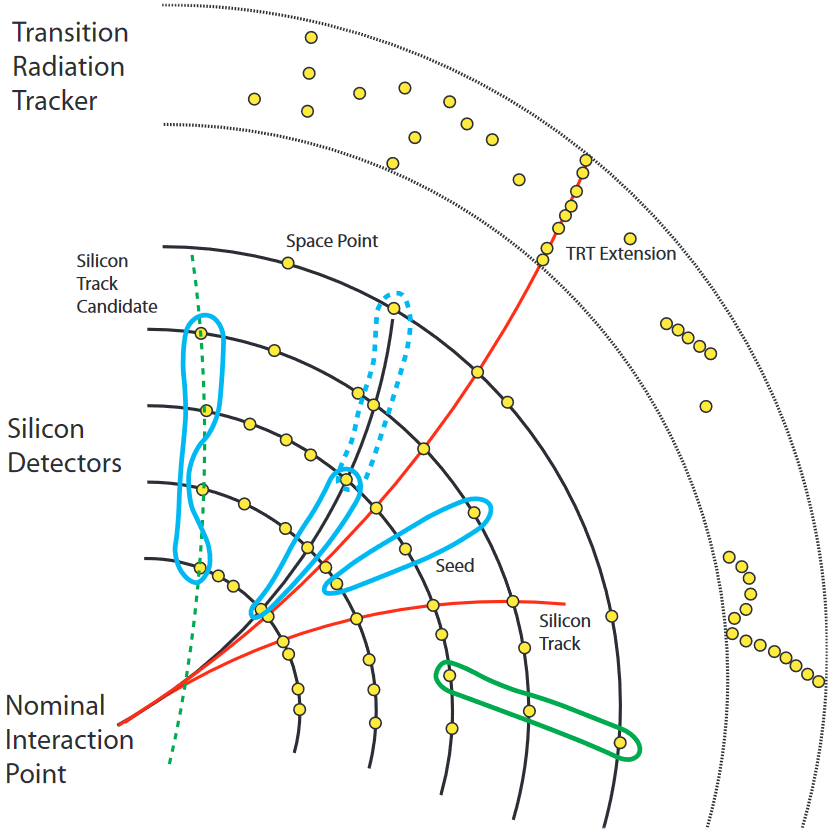
\includegraphics[width=.8\textwidth]{Reconstruction_plots/track.png}
    \caption{An example of track reconstruction~\cite{ATLAS-CONF-2010-072}.
        }
    \label{fig:track_recon}
    \end{centering}
\end{figure}
Track reconstruction is a starting point of physics objects reconstruction,
as it is not only used in reconstruction of charged particles but also
almost every element of reconstruction, such as vertices, pile-up removal,
missing energy and flavour tagging. 
Therefore it is crucial to understand how tracks are reconstructed in ATLAS.
There are 3 stages of reconstruction~\cite{ATLAS-CONF-2012-042}, 
starting with the ``inside-outside''
algorithm, then the ``outside-in'' and finally reconstructing the
TRT-standalone tracks. Figure~\ref{fig:track_recon} shows an illustrative 
view of elements used in tracks reconstruction.
% As shown in Figure~\ref{fig:electron_recon}, a charged particle traverses
% the ID. Space points are formed using the ID information.

The inside-out algorithm starts from assembling clusters from the
raw measurements, from which three-dimensional measurements referred to as
space points are created. They represent the point where the charged particle 
traversed the active material of the ID. 
In the pixel detector, each cluster 
equates to one space-point, while in the SCT, clusters from both sides of a strip
layer must be combined to obtain a three-dimensional measurement.
Once the space-points are created, three sets of space points are combined to seeds. 
A combinatorial Kalman filter~\cite{FRUHWIRTH1987444} is used to 
build track candidates from the chosen seeds by incorporating additional 
space-points from the remaining layers of the pixel and SCT detectors which 
are compatible with the preliminary trajectory. 
A track score is assigned to each track,
which is computed by the $\chi^2$ of fitting the track, intrinsic resolution, 
expected clusters multiplicity, number of holes (missing hits) and track \pt\. 
Ambiguity is solved by selecting the track with the best score.
The final step of the ``inside-out'' algorithm is to extend the silicon
tracks into the TRT. The tracks are fitted again to estimate the final track
parameter (IP, transverse distance from the interaction point) $d_0$, 
distance from the interaction point along the $z$ axis $z_0$,
azimuthal angle $\phi$, polar angle $\theta$ and charge momentum ratio $q/p_T$.
The ``outside-in'' algorithm starts with searching for tracks with segments 
reconstructed in the TRT, and extend the tracks inwards by adding silicon hits. 
Finally, tracks with a TRT segment but no extension into the silicon detectors
are referred as TRT-standalone tracks. Vertices are
matched to interactions by calculating the sum of the weights of the tracks in a vertex matched to
each interaction.


Primary vertices are reconstructed using an iterative vertex finding algorithm \cite{ATLAS-CONF-2012-042}.
Vertex seeds
are obtained from the z-position at the beamline of the reconstructed tracks. An iterative $\chi^2$ fit
is made using the seed and nearby tracks. Tracks displaced by more than $7\sigma$ are used to seed a
new vertex and the procedure is repeated until no additional vertices can be found. The beam spot
position is used as a constraint. Vertices are required to contain at least two tracks. 

starts from 3-point seeds in the silicon detectors and adds hits moving away from the interaction
point using a combinatorial Kalman filter (Iterative algorithm that provides best estimate of the
state based on projection of earlier measurements and current measurement). Ambiguities in the
track candidates are resolved, and tracks are extended into the TRT. This is the baseline algorithm
designed for the efficient reconstruction of primary charged particles. In a second stage, a track
search starts from segments reconstructed in the TRT and extends them inwards by adding silicon
hits. This back-tracking is mainly designed to reconstruct secondaries. Finally tracks with a TRT
segment but no extension into the silicon detectors are referred as TRT-standalone tracks.

\subsection{Electron}
\begin{figure}[bht]
    \begin{centering}	
    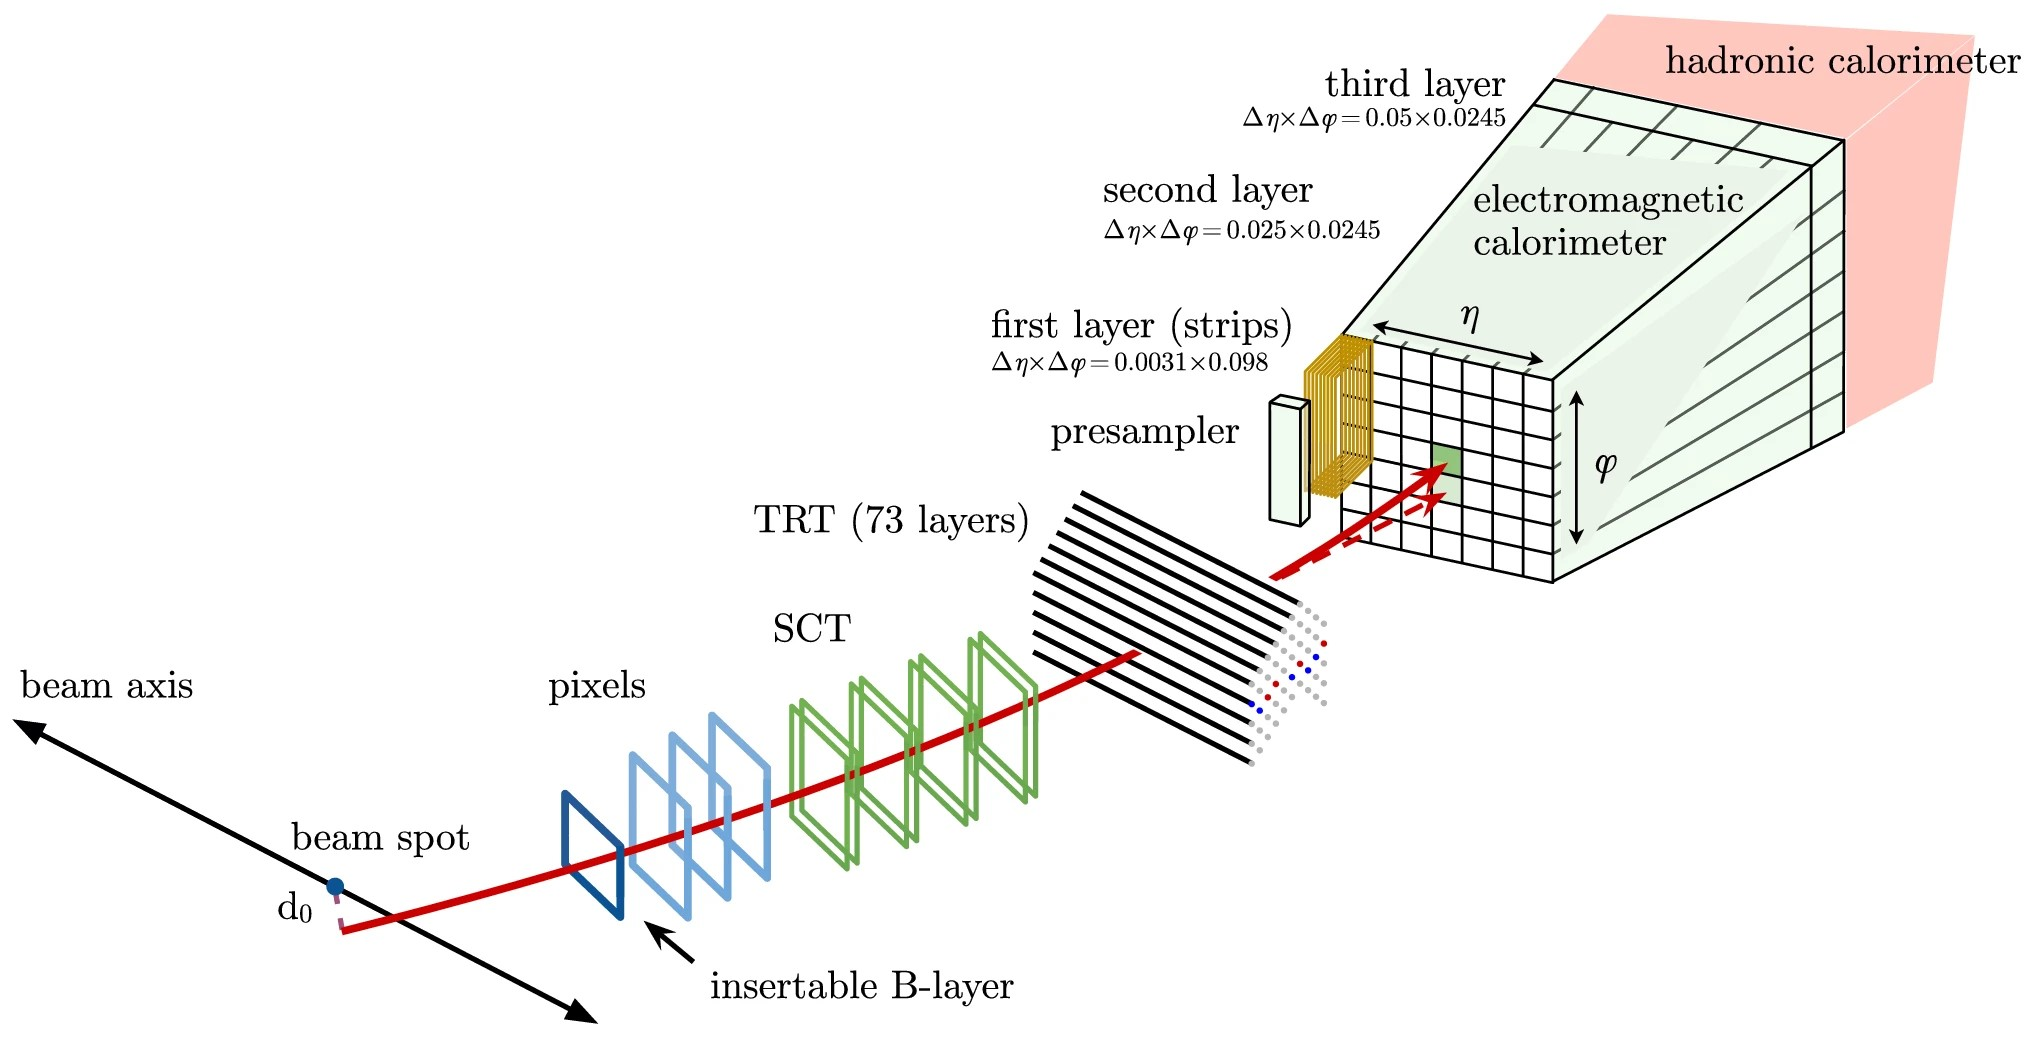
\includegraphics[width=.8\textwidth]{Reconstruction_plots/electron.jpg}
    \caption{A schematic illustration of the path of an electron through the detector. The red trajectory shows the
    hypothetical path of an electron, which first traverses the tracking system (pixel detectors, then silicon-strip detectors
    and lastly the TRT) and then enters the electromagnetic calorimeter. The dashed red trajectory indicates the path of a
    photon produced by the interaction of the electron with the material in the tracking system\cite{PERF-2017-01}.
        }
    \label{fig:electron_recon}
    \end{centering}
\end{figure}
\subsection{Muon}
\subsection{Jet}
